\documentclass[12pt, letterpaper]{article}

\usepackage{graphicx}
\usepackage{parskip} % Disabling paragraph index as it does not fit maths
\usepackage{hyperref} % Usable menu and references
\usepackage{amssymb} % Used to show sets of sumbers, like the real numbers
\usepackage{amsmath} % Used for collumn vectors
\usepackage{tikz} % Used for field diagrams
% Code sourced from https://tex.stackexchange.com/questions/513118/diagram-of-field-theory

\graphicspath{{images}}

\newcommand{\R}{\mathbb{R}}
\newcommand{\C}{\mathbb{C}}
\newcommand{\Q}{\mathbb{Q}}
\newcommand{\Z}{\mathbb{Z}}
\newcommand{\F}{\mathbb{F}}
\newcommand{\N}{\mathbb{N}}

\title{Galois Theory}
\author{Arkadiusz Naks}
\date{2023}

\begin{document}

\begin{titlepage}
  \begin{center}
    \makeatletter
    \vspace*{1cm}
    \Huge
    \textbf{\@title}

    \vspace{0.5cm}
    \Large
    Lecture notes from Galois Theory at Durham University

    \vspace{1.5cm}

    \textbf{\@author}

    % \includegraphics[scale=0.55]{.png}
    \vfill

    \vspace{0.8cm}

    \small
    Based on my understanding of lectures and notes of \\
    \@date{}
  \end{center}
\end{titlepage}

\tableofcontents
\newpage

\begin{section}{Important Definisions}

  A place for short and important definisions

  \textsc{Definision} (Solution by Radicals) \textit{A solution that can be
    expressed by a finite number of basic arithmeic operations a well as
    \(\sqrt[m]{x}\)}

  \textsc{Definision} \textit{For a homomorphism \(\varphi: K \to K'\) and a
    polynomial \(f(x) \in K[x]\) \(\varphi_{*} f(x)\) is the polynomial formed
    by applying \(\varphi\) to \(f(x)\)}

  \textsc{Definision} (Formal Derivative in \(K[x]\)) \textit{For \(f(x) \in
    K[x]\), the derivative is defined as \(D(f) = \sum^{n}_{i = 1} ia_{i}
    x^{i - 1} \in K[x]\)}

\end{section}

\begin{section}{Introduction}

  The primary motivation of Galois Theory is to show that there is no general
  solution for polynomials of degree 5 or higher that can be \textbf{solved by
    radicals}. It can also be used to determine whether a particular given
  equation can be \textbf{solved in radicals} as well as find the algorithm to
  find such solution (which in practice can be extremely complicated).

  \begin{subsection}{Cubics over \(\C\)}

    To find a general solution to an equation
    \(x^{3} + a_{2}x^{2} + a_{1}x + a_{0} = 0\) a substitution
    \(t = x + \frac{a_{2}}{3}\) can be used to eliminate the \(x^{2}\) term
    leading to \[t^{3} + pt + q\] where p and q can be expressed in terms of
    \(a_{2}, a_{1}, a_{0}\), namely \(p = \frac{-a^{2}_{2} + 3a_{1}}{3}\) and
    \(q = \frac{2a^{3}_{2} -9a_{1}a_{2} + 27a_{0}}{27}\). The new equation is
    called a \textbf{reduced} or \textbf{depressed} cubic. Next step is to do a
    substituton of \(p = -3uv\) and \(q = -(u^{3} + v^{3})\). This u and v also
    give a solution \(u + v\) to the \textbf{reduced} cubic. Starting from a
    quodriatic with roots \(u^{3}, v^{3}\), namely
    \((y - u^{3})(y - v^{3}) = 0\) it can be proceesed through the quodratic
    formula
    that \[u^{3}, v^{3} = -\frac{q}{2} \pm \sqrt{\frac{q^{2}}{4}} - \frac{p^{3}}{27}.\]
    which helps optain a solution to the original equation by optaining the
    solutions in t, \(t = u + v\) and substituting back to x. The other two
    solutions can be obtained by multiplying either u or v by
    \(\omega = e^{\frac{2\pi i}{3}}\) and \(\omega^{2}\), (two other results for
    \(x^{3} = 1\)). The pairs of results are
    \(u + v, \omega u + \omega^{2} w, \omega^{2} u + \omega w\).

    The same formulas will give \textbf{solutions in radicals} in other fields
    \(\F_{p}\) for p prime and \(p \geq 5\). They fail for \(p = 2, 3\)
    as they involve divisibily by 2 and 3.

  \end{subsection}

  \begin{subsection}{Quortic over \(\C\)}

    Similarly to a cubic, any given quortic can be changed to a
    \textbf{reduced} form \(t^{4} + pt^{2} + qt + r = 0\). To solve this, it is
    manipulated to obtain a difference (or sum, identical over \(\C\))
    of two squares. This transforms the quortic into two quodritics, each
    containing two anwsers. This can be always achived by introducing a w term
    to get the following equation
    \[(t + w){}^{2} + (p - 2w)t^{2} + qt + (r - w^{2}) = 0\]
    As \((t + w){}^{2}\) is a square for all w (obvious), we need to ensure the
    other part of the equation is also a square. As it is a quodratic, being a
    square implies that it has a repeted root, therefor its determinant is 0.
    Working through the determinant results in the following cubic
    \[w^{3} - \frac{1}{2}pw^{2} - rw + \frac{1}{8}(4pr - q^{2}) = 0\] which
    solved will give an appropriate w and is called the \textbf{cubic resolvent}.
    Only one anwser needs to be obtained from this cubic as the two quodratics
    contain all the anwsers.

  \end{subsection}

  \begin{subsection}{Symmetris}

    One good example of symetries in quodratic roots are complex roots comming
    in conjugate pairs. Another one is very similar, namely real roots come in
    conjugate pairs similar to complex ones if they are structured over
    \(\Q[\sqrt[2]{n}]\) (with n the determinant). Both of these examples
    can be deduced from the quodratic formula.

  \end{subsection}

\end{section}

\begin{section}{Fields}

  \begin{subsection}{Characteristic}

    For a ring homomorphism \(x: \Z \to K\) with K a field and
    \(x: n \to 1_{0} + 1_{1} + \cdots + 1_{n}\), the  \textbf{characteristic}
    of K (\(char(K)\)) is defined as the smalles \(n \geq 1\) s.t. \(x(n) = 0\)
    if such n exists, otherwise \(char(K) = 0\). \\
    \textit{The characteristic of a field is always 0 or prime}

    Iff \(char(K) = 0\) then \(\Q\) is the \textbf{prime subfield} of
    K. \\
    Iff \(char(K) = p\) then \(F_{p}\) is the \textbf{prime subfield} of K.

  \end{subsection}

  \begin{subsection}{Polynomials over Fields}

    For a field K, \(K[x]\) is a ring of polynomials over K,
    \[K[x] = \{a_{0} + a_{1}x + \cdots + a_{n}x_{n} | a_{i} \in K\}{}\]

    \textit{This ring is very similar to \(\Z\)}. It is an integral
    domain as well as an unique factorisation domain.

    \begin{subsubsection}{Irreducibility}

      \textbf{Rational Root Test}: for \(f(x) = a_{n}x^{n} + \cdots + a_{1}x
      + a_{0}\) for all \(a_{i} \in \Z\), if \(f(x)\) has roots in
      \(\frac{b}{c} \in \Q\) then \(b | a_{0}\) and \(c | a_{n}\).

      \textbf{Gauss's Lemma}: suppose \(f(x) \in \Z[x]\) factorises as
      \(f(x) = g(x)h(x)\) where \(g(x), h(x) \in \Q[x]\) then \(\exists r
      \in \Q\) s.t.\ \(rg(x), r^{-1}h(x) \in \Z[x]\). In other
      words, if \(f(x)\) can be factorised in \(\Q\) it also has to be
      factorised in \(\Z\).

      For a map \(\phi: \Z \to F_{p}[x]\), \(f(x) \to \bar{f}(x) =
      f(x) \pmod{p}\), if \(\bar{f}(x)\) is irreducible in \(F_{p}[x]\), then
      \(f(x)\) is irreducible in \(\Q[x]\). This is valid as long as
      p is prime and \(p \nmid a_{n}\). This only goes one way.

      \textit{All of this will work if \(\Z\) is replaced with any ring
        R as long as R is a UFD and \(\Q\) with field of fractions
        \(K = Frac(R)\).}

      \textbf{Eisenstein Criterion}: if \(f(x) = a_{n}x^{n} + \cdots a_{1}x +
      a_{0} \in \Z[x]\) and prime p s.t.\ \(p \nmid a_{n}\),
      \(p | a_{n - 1}, \dots p | a_{1}\) and \(p | a_{0}\) but \(p^{2} \nmid
      a_{0}\) then \(f(x)\) is irreducible in \(\Q\).

      \textit{To generalise Eisenstein to more rings, p has to be prime in R.}

    \end{subsubsection}

  \end{subsection}

  \begin{subsection}{Field Extensions}

    \textit{For a field extension \(L / K\) we generally use Roman letters for
      elements in K and Greek letters for elements in L}.

    \textit{Note: Segment similar to Number Theory (slightly later in the
      term)}.

    A \textbf{field extension}, denoted \(L / K\) is a field L containing a
    subfield K. Despite the notation, this is not a quotient. \\
    A \textbf{simple field extension} is a field extension such that
    \(L = K(x)\), meaning \(L = \{a_{0} + a_{1}x_{1} + \cdots + a_{n}x_{n}
    | a_{i} \in K\}{}\) and \(x_{i}\) are specific elements in L. Generally
    most field extensions are \textbf{simple}. One of the most important things
    about \textbf{field extensions} is how they map between each other.

    For \(S \subset L\) and \(L / K\), \(K(S)\) is called a \textbf{minimal
      subfield} of L that contains both K and S, also called \textbf{K with
      S adjoined}.

    \begin{subsubsection}{Towers of Field Extensions}

      In Galois Theory, towers \(K \subset M \subset L\) s.t.\ K and L are
      fixed and M varies in between are important. One example is \(K =
      \Q\), \(L = \Q(\sqrt{2}, \sqrt{7})\) and M is either
      \(\Q(\sqrt{2}), \Q(\sqrt{7}), \Q(\sqrt{14})\).
      This can be represented with a diagram
      \begin{center}
        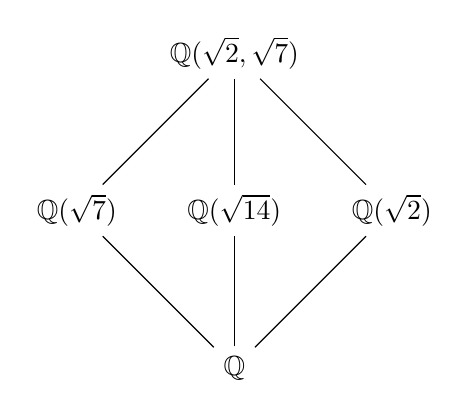
\begin{tikzpicture}

          \node (Q1) at (0,0) {\(\Q\)};
          \node (Q2) at (2,2) {\(\Q(\sqrt{2})\)};
          \node (Q3) at (0,4) {\(\Q(\sqrt{2}, \sqrt{7})\)};
          \node (Q4) at (-2,2) {\(\Q(\sqrt{7})\)};
          \node (Q5) at (0, 2) {\(\Q(\sqrt{14})\)};

          % To add text x:
          % node [pos=0.7, below,inner sep=0.25cm] {};
          \draw (Q1)--(Q2);
          \draw (Q1)--(Q4);
          \draw (Q3)--(Q4);
          \draw (Q2)--(Q3);
          \draw (Q1)--(Q5);
          \draw (Q3)--(Q5);

        \end{tikzpicture}
      \end{center}
      \(\Q(\sqrt{2}, \sqrt{7}) / \Q\) is also a
      \textbf{simple extension} as it can be writen as \(\Q()\).

    \end{subsubsection}

  \end{subsection}

  \begin{subsection}{Algebraic Elements}

    For a field extension \(L / K\) and \(\theta \in L\), \(\theta\) is called
    \textbf{algebraic} if there exists a non-zero polynomial \(f(x) \in K[x]\)
    s.t.\ \(f(\theta) = 0\), otherwise it is called \textbf{transcendental
      over} K. \\
    \textit{For a field \(K(t)\), t is always \textbf{transcendental} over K}.

    Furthermore for the same field extention and element \(\theta \in L\),
    \[I_{K}(\theta) = \{f(x) \in K[x] | f(\theta) = 0\}.\] This makes
    \(I_{K}(\theta)\) a subset of all polynomials in K for which \(\theta\) is
    a root. This subfield is clearly \(\{ 0 \}\) if \(\theta\)
    \textbf{transcendental}. On the other hand, if \(\theta\) is
    \textbf{agebraic}, \(\exists m(x) \in K[x]\) which generates the subset.
    This \(m(x)\) is unique, irreducible and monic in \(K[x]\). This subset is
    an \textbf{ideal} in \(K[x]\). \\
    The polynomial \(m(x)\) is called the minimal polynomial of \(\theta\), and
    the degree of \(\theta = \deg m(x)\). As \(m(x)\) generates the ideal, it
    is the only irreducible element of it. This means that any irreducible
    monic polynomial is a minimal polynomial for all its roots.

  \end{subsection}

  \begin{subsection}{Constructing Simple Field Extensions}

    \(f(x) \in K\) irreducible over K \(\iff K[x]/(f(x))\) is a field (for
    \(f(x) \neq 0\)). Furthermore for \(m(x) \in K[x]\) monic and irreducible
    polynomial:
    \begin{itemize}
      \item \(K_{m} = K[x] / (m(x))\) is a field extension of K
      \item For a map \(\pi : K[x] \to K_{m}\) s.t.\ \(f(x) \mapsto f(\theta)\)
            and \(\theta = \pi(x)\). Then \(\theta\) has minimal polynomial
            \(m(x)\) and \(K_{m} = K(\theta)\)
    \end{itemize}
    This \(K_{m}\) field extension is the minimal field containg K and the root
    of \(m(x)\), as well as n dimentional vector space over K, with \(n =
    \deg m(x)\).

    For two field extensions \(L_{1} / K\) and \(L_{2} / K\) and \(\varphi:
    L_{1} \to L_{2}\) a field homomorphism, then \(\varphi\) is called a
    \textbf{K-homomorphism} if \(\forall a \in K \; \varphi(a) = a\). It can
    be said that \(\varphi\) \textbf{fixes} K. If it is an isomorphism of fields
    then it is called \textbf{K-isomorphism}. (Also K-automorphism is a
    K-isomorphism)

    Take \(K_{m} / K\) with \(\pi\) and \(\theta\) as above, then for \(L / K\)
    with \(\theta' \in L\) satisfying \(m(\theta') = 0\), \(K_{L}(\theta')\) is
    the minimal subfield of L containg K and \(\theta'\), there exists an
    unique K-isomorphism \(\varphi: K_{m} \to K_{L}(\theta')\) s.t.\
    \(\varphi(\theta) = \theta'\).

    This is somewhat easier to denote if \(\theta\) is \textbf{transcendental}.
    In such cases there is a unique K-isomorphism \(\varphi: K(t) \to
    K(\theta)\) s.t.\ \(\varphi(t) = \theta\).

  \end{subsection}

  \begin{subsection}{Some Interesting Simple Extensions}

    \(F_{9} \neq \Z / 9\) is defined as \(\Z / 3 (\theta)
    = F_{3}(\theta) = F_{3} / (x^{2} - 2) = F_{9}\) where \(\theta^{2} = 2\).
    This is actually the same as \(F_{3}(i)\) with i as ususal.

    Similarly \(F_{4} \neq \Z / 4\) is defined as
    \(F_{4} = F_{2} / (x^{2} + x + 1) = F_{2}(\theta)\) for \(\theta^{2} =
    \theta + 1\).

    For any q power of a prime, there exists \(F_{q}\) (unique up to
    isomorphism) with q elements. These fields are called \textbf{Galois
      fields}. \textit{More next term}

  \end{subsection}

  \begin{subsection}{Degrees of Field Extensions}

    For an arbitrary field extension \(L / K\) L is a vector space over K. \\
    \textit{This construction essentially removes multiplication for elements
      of L outside of K. This can actually be very useful}.

    The degree of \(L / K\) is the dimention of L over K (size of the basis)
    and is denoted as \([L : K]\). When \(\theta\) is algebraic over K,
    \([K(\theta) : K] = n\). If \([L : K] < \infty\), then it is finite and
    all elements of L are \textbf{algebraic} over K. This is called an
    \textbf{algebraic extension}. If \(\theta = t\) (\textbf{indeterminate}) or
    is \textbf{transcendental}, \([L : K] = \infty\). \\
    \textit{There are infinite field extensions with no transcendental
      elements, which cannot be generated by adjoining finitely many algebraic
      elements}.

    For a tower of extensions \(K \subset M \subset L\), \([L : K] =
    [L : M] \times [M : K]\) and \([L : K] < \infty \Rightarrow [L : M],
    [M : K] < \infty\). This also means that for a field K and \(\alpha,
    \beta\) algebraic over K, \([K(\alpha, \beta) : K] \leq
    [K(\alpha) : K] \times [K(\beta) : K]\).

  \end{subsection}

\end{section}

\begin{section}{Galois Extensions}

  \begin{subsection}{Nice Fields}

    \begin{subsubsection}{Splitting Fields}

      A \textbf{spliting field} of \(f(x) \in K[x]\) contains all roots of
      \(f(x)\) and is \textbf{minimal}. For \(L / K\), L is the \textbf{spliting
        field} if \(f(x) = c(x - \theta_{1}) \cdots (x - \theta_{n})\) with all
      \(\theta_{i} \in L\) (for \(c \in K, \; c \neq 0\)). Every polynomial in K
      has exacly one splitting field with \([L : K] \leq n!\) (with n the degree
      of the polynomial). An isomorphism \(\varphi: K \to K'\) can be extended
      to an isomorphism \(\sigma: L \to L'\) with L and L' begin spliting fields
      of K and K' and polynomials \(f(x)\) and \(f'(x) = \varphi_{*}(f(x))\).
      This is a property of a field extension for a single polynomial.

    \end{subsubsection}

    \begin{subsubsection}{Normal Fields}

      A \textbf{normal} extension \(L / K\) is s.t.\ for any \(f(x) \in K[x]\)
      irrdecucable, it is \textbf{split} by L.
      A much less strict condition is \(L / K\) extention is only
      \textbf{finite} and \textbf{normal} iff L is \textbf{splitting} for one
      \(f(x) \in K[x]\). This is a property of the entire field extension. \\
      A \textbf{normal closure} N of \(L / K\) is defined as \(K \subset L
      \subset N\) s.t.\ \(N / K\) \textbf{normal} and N is minimal. A finitie
      field extension always has unique \textbf{closure}.

    \end{subsubsection}

    \begin{subsubsection}{Seperable Fields}

      An element \(\theta \in L\) is \textbf{seperable over} K if its minimal
      polynomial has no repeated roots in its \textbf{spliting} field. If all
      elements of L are \textbf{seperable} over K, the whole extension is
      called \textbf{seperable}.

      A finite extension \(L / K\) is \textbf{seperable} if:
      \begin{itemize}
        \item \(char(K) = 0\)
        \item \(char(K) = p\) and \(K = K^{p}\), i.e.\ ever \(a \in K\)
              can be writen as \(b^{p}\) with \(b \in K\)
        \item \(char(K) = p\) and \(p \nmid [L : K]\)
      \end{itemize}
      If a field satisfies condition one or two, it is called \textbf{perfect}.

      A simpler condition for the whole field to be \textbf{seperable} is for
      its minimal polynomial has no repeated roots in its \textbf{spliting}
      field. For a tower \(K \subset M \subset L\) \(L / K\) is \textbf{seperable}
      iff both \(L / M\) and \(M / K\) are. Being seperable and finite also
      implies being \textbf{simple}. \\

      \end{subsubsection}

  \end{subsection}

  \begin{subsection}{Automorphisms}

    A set of K-automorphisms of \(L / K\) forms a group with composition,
    denoted as \(Aut(L / K\)). For \(L = K(\theta)\) with \(\theta\) algebraic
    and \(\deg(\theta) = n\), \(|Aut(L / K)| \leq n\). This changes to an
    equality when \(p_{\theta}(x)\) has n distinct roots in L. This can be
    generalised for any field extension \(L / K\); \[|Aut(L / K)| \leq [L : K]\]
    with equality iff \(L / K\) is \textbf{normal} and \textbf{seperable}.

  \end{subsection}

  \begin{subsection}{Definision}

    If a field extension \(L / K\) is both \textbf{normal} and
    \textbf{seperable}, it is called a \textbf{Galois Extension}. Its
    automorphisms group, or \textbf{Galois group}, is denoted as \(Gal(L / K)\).
    This means that \(|Gal(L / K)| = [L : K]\).

    For a field L and a group of automorphisms G, a \textbf{fixed field} of G
    \(L^{G} = \{ \alpha \in L | \varphi(\alpha) = \alpha \; \forall \varphi \in
    G\}\) is a subset of L which all the automorphisms fix. If G is finite,
    \(L^{G} \subset L\) and furthermore \([L : L^{G}] = |G|\). This implies
    that for a Galois extension \(L / K\), \(L^{Gal(L / K)} = K\). Also for \(H
    \subset Gal(L / K)\), \(K \subset L^{H} \subset L\).

    \begin{subsubsection}{Fundamental Theorem of Galois Theory}

      For Galois extension \(L / K\), \[\mathcal{F} = \{ intermidiate \; fields
        \; of \; L / K \} \; and \; \mathcal{G} = \{ subgroups \; of \; Gal(L / K)
      \},\] \(\exists \Gamma : \mathcal{F} \to \mathcal{G}\) with \(M \mapsto
      Gal(L / M)\). Importantly all \(L / M\) for \(M \in \mathcal{F}\) are
      Galois extensions. Meanwhile \(M / K\) while not neccessarily Galois can
      make \(Gal(M / K)\) a \textbf{quotient} of \(L / K\) under the right
      conditions. There also exists \(\Phi: \mathcal{G} \to \mathcal{F}\)
      maps \(H \mapsto L^{H}\). \\
      This maps are \textbf{mutually inverse bijections} (\textbf{Galois
        Correspondance}).

      For all \(M \in \mathcal{F}, H \in \mathcal{G}\) all extensions \(L / M\) as
      well as \(L / L^{H}\) are \textbf{Galois} with \(| Gal(L / M) | = [L : M]\)
      and \(Gal(L / L^{H}) = H\).

      For the second part of the tower \(K \subset M \subset L\), if it exists,
      \(| Gal(M / K) | = [M : K] = \frac{[L : K]}{[L : M]} = \frac{| G |}{| H |
      }\) with \(G = Gal(L / K)\) and \(H = Gal(L / M)\).
      The following are equivelant
      \begin{itemize}
        \item \(M / K\) is \textbf{Galois}
        \item \(\sigma(M) = M \; \forall \sigma \in G\)
        \item H is a \textbf{normal subgroup} of G
        \item \(Gal(M / K) \cong G / H\)
      \end{itemize}

    \end{subsubsection}

  \end{subsection}

\end{section}

\begin{section}{Cyclotomic Field Extensions}

  For \(K \subset L\) Galois, \(n \geq 1\) and \(Gal(L / K) \cong \Z_{n}\),
  then L is called a \textbf{cyclic} extension of K of degree n.

  \begin{subsection}{Roots of Unity}

    \(\zeta \in K^{\times}\) is the n-th primitive root of unity if \(\zeta^{n}
    = 1\) and \(\zeta^{m} \neq 1 \; \forall 0 < m < n\). If \(char(K) = p\),
    then K does not contain the p-th root of unity. For \(K = \C\),
    \(\zeta_{n} = \cos(2 \pi / n) + i \sin(2 \pi / n) = e^{2 \pi / n}\).

    \(\mu(K)\) denotes the group of all roots of unity in \(K^{\times}\).
    As all finite subgroups of \(K^{\times}\) are cyclic, \(\mu(K)\) is cyclic.
    Also any finite cyclic group of order n appears as a subgroup of
    \(K^{times}\) iff K contains the n-th primitive root of unity. \(\mu(K)\)
    is generated by \(\zeta\) where \(\zeta\) is the n-th primitive root of
    unity and there are no primitive roots of unity in K of order bigger than
    n.

  \end{subsection}

  \begin{subsection}{Definision}

    For \(n \geq 1\) let \(\zeta_{n}\) denote the n-th primitive root of unit
    in \(\C\), then the field extension \(\Q(\zeta_{n})\) of \(\Q\) is called
    the n-th \textbf{cyclotomic} field extension. This are always Galois over
    \(\Q\).

    \(\Phi_{n}(x)\) denotes the minimal polynomial of \(\zeta_{n}\) over
    \(\Q\). \([\Q(\zeta_{n}) : \Q] = \varphi(n)\) with \(\varphi\) the Euler
    function (look ENT notes). \\
    \(\Phi_{n}(x)\) can be defined by \(x^{n} - 1 = \prod_{i | n} \Phi_{i}\),
    which can be rearanged to get \(\Phi_{n}(x)\). If \(n = p\) prime,
    \(\Phi_{n}(x) = x^{p - 1} + \cdots + x + 1\). For \(n = p^{s}\),
    \(\Phi_{n}(x) = \Phi_{p}(x^{p^{s - 1}})\).

    \(Gal(\Q(\zeta_{n} / \Q)) \cong \Z^{\times}_{n}\). This means that for p
    prime, \(Gal(\Q(\zeta_{p})) \cong \Z_{p - 1}\).

    For an odd n, \(\mu(\Q(\zeta_{n}))\) is a cyclic group of order 2n and it
    is generated by \(-\zeta_{n}\). For n even, \(\mu(\Q(\zeta_{n}))\) is of
    order n and generated by \(\zeta_{n}\). \\
    If \(\gcd(m, n) = 1\), \(\Q(\zeta_{m}, \zeta_{n}) = \Q(\zeta_{mn})\). More
    generally for any \(m, n, M = lcm(m, n)\), \(\Q(\zeta_{m}, \zeta_{n}) =
    \Q(\zeta_{M})\).

    \begin{subsubsection}{Prime P}

      In this section p is always prime and \(p > 2\).

      \(\{\zeta_{p}, \dots , \zeta^{p - 1}_{p}\}\) is a good \(\Q\) baisis for
      \(\Q(\zeta_{p})\) as it does not change under any group action in
      \(Gal(\Q(\zeta_{p}) / \Q)\). \\
    \end{subsubsection}

  \end{subsection}

\end{section}

\begin{section}{Cyclic Field Extensions}

  \begin{subsection}{Primitive Roots}

    In a filed K, \(\zeta \in K^{\times}\) is the n-th primitive root of unity
    if \(\zeta^{n} = 1\) but for all \(0 < m < n\) \(\zeta^{m} \neq 1\). For
    any k \(\zeta^{k} = \zeta^{k \pmod{n}}\). \\
    For any n, \(\zeta_{n}\) represents the n-th primitive root.

    The subgroup of K, denoted \(\mu(K)\) of all primitive roots of unity is
    cyclic, normal and finite.

    \begin{subsubsection}{Minimal Polynomial}

      \(x^{n} - 1 = \prod_{n_{1} | n} \phi_{n_{1}}(x)\) where \(\phi_{m}\) is
      the minimal polynomial of \(\zeta_{m}\). This implies that the degree of
      \(\phi_{m} = \varphi(m)\) with \(\varphi\) the Euler function. \\
      If m is prime, \(\phi_{m}(x) = x^{m - 1} + \cdots + x + 1\) and if
      \(m = p^{s}\) with p prime \(\phi_{m}(x) = \phi_{p}(x^{p^{s - 1}})\).

    \end{subsubsection}

  \end{subsection}

  \begin{subsection}{Cyclotomic Definision}

    The field extension \(\Q(\zeta_{n} / \Q)\) is  the n-th \textbf{cyclotomic}
    field extenstion. These are always \textbf{Galois}.

    \begin{subsubsection}{Galois Group}

      \(Gal(\Q(\zeta_{n}) / \Q) = G \cong \Z^{\times}_{n}\), being the group of
      numbers mod n with respect to multiplication. If \(n = p\) prime, G is
      \textbf{cyclic} of order \(p - 1\). \\
      G can still be cyclic for not prime n.

      The best basis for \(\Q(\zeta_{p})\) is
      \((\zeta_{p}, \zeta^{2}_{p}, \dots , \zeta^{p - 1}_{p})\).

      For \(x \in \Q(\zeta_{p})\) let \(X = \{g(x) | g \in G\}\)
      (discounting the duplicates) \([\Q(x) : \Q] = | X | \). The minimal
      polynomial for such x over \(\Q\) is \(f(t) = \prod_{i \in X} (t - i)\).

    \end{subsubsection}

    \begin{subsubsection}{Subfields}

      Any subfield of \(\Q(\zeta_{n})\) is automatically \textbf{Galois} over
      \(\Q\). \\
      For any divisor d of \(p - 1\), \(\Q(\zeta_{p})\) contains exacly one
      subfield of that degree. There are no subfields of degree m s.t.
      \(m \nmid p\). The quodratic subfield (\(p \neq 2\)) is of the form
      \(\Q(\sqrt{m})\) where m is p if \(p \equiv 1 \pmod{4}\), otherwise
      \(m = -p\). \\

    \end{subsubsection}

  \end{subsection}

  \begin{subsection}{Degree 2}

    For any field K and \(L / K\) Galois, \(G = \Z_{2} = \{e, \tau\}\) where
    \(\tau^{2} = e\). Furthermore if \(char K \neq 2\) then any \textbf{cyclic}
    Galois extension is of the form \(L = K(\sqrt{a})\) where
    \(a \in K^{\times}\) and squarefree. If \(K(\sqrt{a_{1}}) =
    K(\sqrt{a_{2}})\), \(a_{1} \equiv a_{2} \pmod{s}\) for some
    \(s \in K^{\times}\) (squares in K). \\
    If \(a_{1}, \dots , a_{n}\) independent mod any prime, \(K(\sqrt{a_{1}},
    \dots , \sqrt{a_{n}})\) is of degree \(2^{n}\) with galosi group
    \(G \cong \Z^{n}_{2}\). The Galois group is only of that form if L is of
    that form.

  \end{subsection}

  \begin{subsection}{Degree n}

    If K contains a primitive n-th root of unity \(\zeta_{n}\) and
    \(\exists a \in K^{\times}\) s.t.\ \(a\) is not \(\alpha^{d}\) for d one of the
    divisors of n, then \(L = K(\sqrt[n]{a})\) is \textbf{cyclic} extension  of
    degree n and \(f(x) = x^{n} - a\), \(f(x) \in K[x]\) is
    \textbf{irreducible}. \\
    This also holds the other way, if \(L / K\) is cyclic degree n and K
    containt \(\zeta_{n}\), then \(\exists a \in K^{\times}\) with \(L =
    K(\sqrt[n]{a})\).

  \end{subsection}

  \begin{subsection}{Lagrange Resolvant}

    Let \(K(\sqrt[n]{a}) = K(\theta) = L / K\) be galois cyclic of degree n, and
    \(\tau \in Gal(L / K) = G\) s.t.\ \(\langle \tau \rangle = G\). Then for any
    \(b_{0} \in L\) with \(\tau(b_{0}) = b_{1}\) and so on
    (\(\tau(b_{i}) = b_{(i + 1) \pmod{n}}\)),
    \[\theta_{b_{0}} = b_{0} + \zeta^{-1}_{n} b_{1} + \cdots +
      \zeta^{-(n - 1)}_{n} b_{n - 1}\] is called the \textbf{Lagrange resolvent}
    for \(b_{0}\).

    Note that \(\tau(\theta) = \theta \zeta'\) for \(\zeta'\) some root of unity
    and \(\tau(\theta_{b_{0}}) = \theta_{b_{0}} \zeta_{n}\).

    There always exists \(b_{0}\) s.t.\ \(\theta_{b_{0}} \neq 0\).

  \end{subsection}

\end{section}

\begin{section}{Finite Fields}

  \begin{subsection}{Introduction}

    For K a finite field, then there exists some prime p, s.t.\
    \(\F_{p} \subset K\), meaning K has a characteristic of p. This emans that
    for \(1 \in K\), \(p \times 1 = 0 \in K\). The number of elements in such
    field is \(| K | = p^{n}\) for some \(n \in \N\). \\
    For any \(n \in \N\), there exists K s.t.\ \(| K | = p^{n}\).

    Any two finite fields K, L are isomorphic iff \(| K | = | L |\). These are
    usually denoted as \(\F_{q = p^{n}}\).

    \begin{subsubsection}{Galois}

      \(\F_{q}\) is always Galois over \(\F_{p}\) with the Galois group G
      isomorphic to \(\Z_{n}\). \\
      This is because it is splitting for \(x^{q} - x\).

    \end{subsubsection}

  \end{subsection}

  \begin{subsection}{Irreducable}

    Let \(Irr_{\F_{p}}(N)\) be the set of all monic irreduciable polynomials in
    \(\F_{p}[x]\) of degree N. Then for \(q = p^{N}\) \[N | Irr_{\F_{p}}(N) |
      = | \{ \alpha \in \F_{q} | \F_{p}(\alpha) = \F_{q}\} |.\] Essentially the
    number of irreduciable polynomials is related to the number of elements
    which can be adjoined to \(\F_{p}\) to make a field of the degree of the
    polynomial. \\
    \(\F(\alpha) \neq \F_{q} \iff \F(\alpha) \subsetneq \F_{q}\).

  \end{subsection}

\end{section}

\begin{section}{General Polynomials}

  \begin{subsection}{Symmetric Funtions}

    \begin{subsubsection}{Setup}

      For K a field of characteristic 0 (or p, where p coprime to \(n!\)), let
      \(L = K(x_{1}, \dots , x_{n})\) be a field of rational function in n
      \textbf{independent} variables (with \(K = L^{S_{n}}\)). Then if \(L / K\)
      is Galois, \(Gal(L / K) = S_{n}\), where for \(\tau =
      \begin{pmatrix}
        1 && 2 && \dots && n \\
        m_{1} && m_{2} && \dots && m_{n}
      \end{pmatrix}\) acts on L \(x_{i} \mapsto x_{m_{i}}\).

    \end{subsubsection}

    \begin{subsubsection}{Elementary Symmetric Functions}

      They are defined as \(\sigma_{1} = \sum^{n}_{i = 1} x_{i}\),
      \(\sigma_{2} = \sum_{1 \leq i < j \leq n} x_{i} x_{j}\),
      \(\sigma_{3} = \sum_{1 \leq i < j < k \leq n} x_{i} x_{j} x_{k}\),
      and so on. (\(\sigma_{i}\) actually means \(\sigma_{i}(L)\)). \\
      Clearly any \(\sigma_{i}(L) \in L\). Also (not as clearly)
      \(k(\sigma_{1}, \dots , \sigma_{n}) = K\)

      This means that \(k[\sigma_{1}, \dots , \sigma_{n}] =
      k[x_{1}, \dots , x_{n}]^{S_{n}} (= P)\) and therefor
      \textbf{any symmetric polynomial can be expressed as a polynomial in ESFs}

      \(f(T) = (T - x_{1})(T - x_{2}) \dots (T - x_{n}) =
      T^{n} - \sigma_{1} T^{n - 1} + \sigma_{2} T^{n - 2} + \cdots +
      (-1)^{n}_{\sigma_{n}}.\)

    \end{subsubsection}

    % Review usefullness
    \begin{subsubsection}{Calculations}

      For a symmetric polynomial \(p(x_{1}, \dots , x_{n}) \in P\) it can be
      said that
      \[p = \sum_{\textbf{a}} \alpha_{\textbf{a}} x^{a_{1}}_{1} \dots x^{a_{n}}_{n}\]
      for \(\alpha_{\textbf{a}} \in k\) and \(\textbf{a} \in k^{n}\) (will be in
      \(\Z\) most of the time??).

      Then to compute the symmetric polynomial \(P(x)\) in terms of elementary
      functions, take the \textbf{monomialy} biggest term
      \(x^{a_{1}}_{1} \dots x^{a_{n}}_{n}\) and define \(p_{1} = p - r\) where
      \[r = \alpha_{\textbf{a}} \sigma^{a_{1} - a_{2}}_{1} \dots
        \sigma^{a_{n - 1} - a_{n}}_{n - 1} \sigma^{a_{n}}_{n}.\]
      Apply the algorithm from the beggining on \(p_{1}\) if \(p_{1} \neq 0\).

    \end{subsubsection}

  \end{subsection}

  \begin{subsection}{Degree n}

    For some fields k, \(K = k(\sigma_{1}, \dots , \sigma_{n})\) and
    \(L = k(X_{1}, \dots , X_{n})\) and an irreducable polynomial \(f(X) =
    X^{n} - \sigma_{1} X^{n - 1} + \sigma_{2} X^{n - 2} - \cdots (-1)^{n} \sigma_{n}\)
    with roots \(X_{1}, \dots , X_{n}\).

  \end{subsection}

  \begin{subsection}{Degree 2}

    Use the normal quodratic formula and \(Gal(K(X_{1}, X_{2}) / K) = \Z_{2}\).

  \end{subsection}

  \begin{subsection}{Degree 3}

    \begin{subsubsection}{Solutions}

      Compute the quodratic resolvant of \(f(X)\). This is \(g(U) \in K[U]\)
      \(U^{2} + aU + b\) where \[a = \frac{1}{27} (2 \sigma^{3}_{1} -
        9 \sigma_{1} \sigma_{2} + 27 \sigma_{3})\] and \(b = \frac{1}{9^{3}}
      (\sigma^{2}_{1} - 3 \sigma_{2})^{3}\).

      Then find the roots of \(g(U)\) \(U_{1}, U_{2}\), define
      \(\theta_{1} = \sqrt[3]{U_{1}}\) and \(\theta_{2}\) s.t.
      \(\theta^{3}_{1} \theta^{3}_{2} = b\) and
      \(X_{1} = \frac{\sigma_{1}}{3} + \theta_{1} + \theta_{2}\),
      \(X_{2} = \frac{\sigma_{1}}{3} + \theta_{1} \rho + \theta_{2} \rho^{2}\),
      \(X_{3} = \frac{\sigma_{1}}{3} + \theta_{1} \rho^{2} + \theta_{2} \rho\).
      \\
      Where \(\rho\) is the third root of unity.

    \end{subsubsection}

    \begin{subsubsection}{Galois Group}

      The group is either \(S_{3}\) or \(A_{3}\). To resolve this, calculate the
      discriminant \[\Delta_{0}  = -27 (b^{2} - 4c)\] with a and b the
      coefficiants of the resolvant polynomial. \\ Then
      \begin{itemize}
        \item \(\Delta_{0} \in K^{\times 2} \iff Gal(L / K) = A_{3}\)
        \item Otherwise \(Gal(L / K) = S_{3}\)
      \end{itemize}

    \end{subsubsection}

    \begin{subsubsection}{Reduced Cubic}

      A reduced cubic is \(h(X) = X^{3} + aX + b\). Its quodracit resolvent is
      \(U^{2} + bU - \frac{a^{3}}{27}\). \\
      Also \(\Delta_{0} = -4a^{3} - 27b^{2}\)

    \end{subsubsection}

  \end{subsection}

  \newpage

  \begin{subsection}{Degree 4}

    \begin{subsubsection}{Solutions}

      First compute the cubic resolvant of \(f(X)\). This is \(g(U) \in K[U]\),
      \(g = U^{3} + aU^{2} + bU + c\) where \[a = -\frac{3}{4} \sigma^{2}_{1} +
        2 \sigma_{2},\]
      \[b = \frac{3}{16} \sigma^{4}_{1} - \sigma^{2}_{1} \sigma_{2} +
        \sigma^{2}_{2} + \sigma_{1} \sigma_{3} - 4 \sigma_{4},\]
      \[c = -(d){}^{2} = -(\frac{\sigma^{3}_{1}}{8} -
        \frac{\sigma_{1} \sigma_{2}}{2} + \sigma_{3}){}^{2}.\]

      Then compute the roots \(U_{1}, U_{2}, U_{3}\) of \(g(U)\) can be computed
      and \(\theta_{i} = \pm \sqrt{U_{i}}\) where the sign is chosen such that
      \(\theta_{1} \theta_{2} \theta_{3} = -d\).

      Finally \(X_{1} = \frac{1}{2} (\theta_{1} + \theta_{2} + \theta_{3})\)
      and other \(X_{i}s\) are the same sums with odd numbers of odd signs (the
      order does not matter).

    \end{subsubsection}

    \begin{subsubsection}{Galois Group}

      The Galois group of L depends on the group of
      \(\tilde{L} = k(U_{1}, U_{2}, U_{3})\). If \(g(x)\) is irreducable,
      \begin{itemize}
        \item \(Gal(\tilde{L} / K) = S_{3} \Rightarrow Gal(L / K) = S_{4}\)
        \item \(Gal(\tilde{L} / K) = A_{3} \Rightarrow Gal(L / K) = A_{4}\)
      \end{itemize}
      On the other hand if it is reducable
      \begin{itemize}
        \item \(U_{1}, U_{2}, U_{3} \in K \Rightarrow Gal(L / K) = \Z_{2}
              \times \Z_{2}\)
        \item \(U_{1} \in K \Rightarrow \) \\
              \(Gal(\tilde{L} / K) = \{e, \tau\}\) then for \(\alpha \in
              \tilde{L}^{\times}\) and \(\bar{\alpha} = \tau(\alpha)\) s.t.\
              \(\alpha, \bar{\alpha} \notin \tilde{L}^{\times 2}\)
              \begin{itemize}
                \item \(\alpha \bar{\alpha} \in K^{\times 2}
                      \Rightarrow Gal(L / K) = \Z_{2} \times \Z_{2}\)
                \item \(\alpha \bar{\alpha} \in \tilde{L}^{\times 2}
                      \backslash K^{\times 2} \Rightarrow \Z_{4}\)
                \item \(\alpha \bar{\alpha} \notin \tilde{L}^{\times 2}
                      \Rightarrow Gal(L / K) = D_{4}\)
              \end{itemize}
      \end{itemize}

    \end{subsubsection}

  \end{subsection}

\end{section}

\end{document}
